%%!TEX root = ./UserManual.tex
\chapter{Visualiser}
\label{chap:visualiser}


%%%%%%%%%%%%%%%%%%%%%%%%%%%%%%%%%%%%%%%%%%%%%%%%%%%%%%%%%%%%%%%%
% Overview
%%%%%%%%%%%%%%%%%%%%%%%%%%%%%%%%%%%%%%%%%%%%%%%%%%%%%%%%%%%%%%%%
\section{Overview}
\label{section:overview}

\paragraph{} The Stride software includes a visualisation tool with which the disease spreading can be shown on a geographical map. When the visualiser is opened, the user is presented with a geographical map, a sidebar to the left and a toolbar on top. An overview can be seen in figure \ref{fig:screenshot_overview}

The toolbar contains various controls:
\begin{itemize}
\item Open file: Opens a open file dialog.
\item Save file: Opens a save to image file dialog.
\item Select Radius: Opens the radius selection dialog.
\item Select Rectangle: Opens the rectangle selection dialog.
\item Play-button: Enables/disables the automatic playback of the simulation results.
\item Timestep-slider: Allows the user to select a certain timestep of the simulation.
\item Health status dropdown: Allows the user to select a health status that is to be displayed.
\end{itemize}

%%%% IMAGE: overview

\begin{figure}[H]
\centering
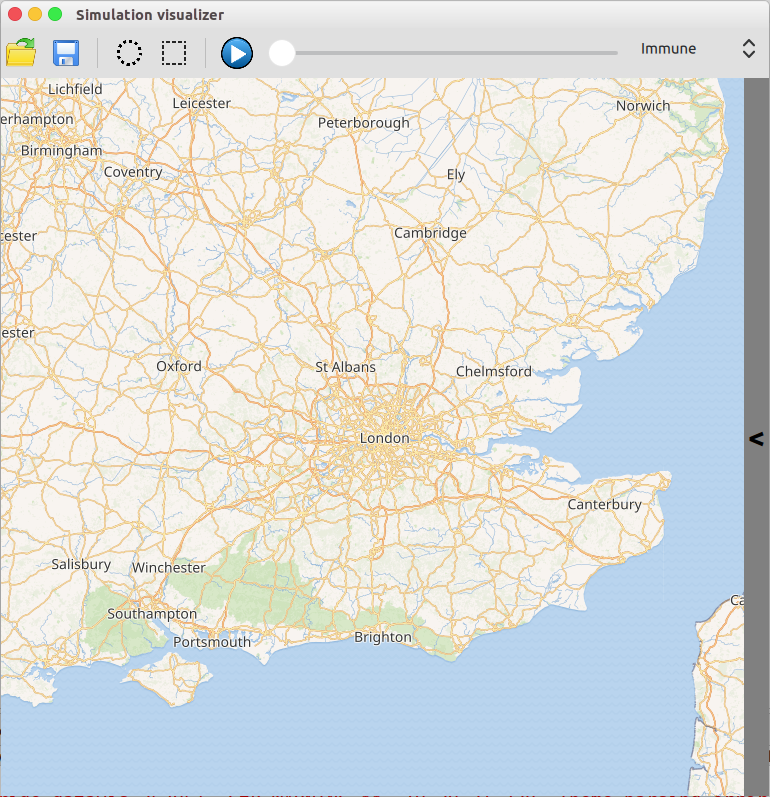
\includegraphics[width=0.7\textwidth,keepaspectratio]{images/overview.png}
\label{fig:screenshot_overview}
\caption{Overview of the visualisation tool}
\end{figure}

%%%%%%%%%%%%%%%%%%%%%%%%%%%%%%%%%%%%%%%%%%%%%%%%%%%%%%%%%%%%%%%%
% Epioutput
%%%%%%%%%%%%%%%%%%%%%%%%%%%%%%%%%%%%%%%%%%%%%%%%%%%%%%%%%%%%%%%%
\section{Epioutput}
\label{section:epioutput}
The visualiser is capable of loading files with epidemiological data, generated using stride. These files are referred to as 'epioutput' files, and can be used in three formats. They are generated by stride if provided with an appropriate configuration file. In order to generate an epioutput file, there are three parameters that can be set in the configuration file:

\begin{compactdesc}
\item [output\_epi] \ \\
    This parameter takes a boolean value indicating whether or not epioutput should be generated. Defaults to \emph{false}.
\item [output\_epi\_type] \ \\
    This parameter indicates the desired format for the epioutput. Currently supports '\emph{json}', '\emph{hdf5}' and '\emph{proto}'.
\item [output\_epi\_interval] \ \\
    This parameter can be used to set an interval between recorded timesteps, e.g. and interval of 10 will capture the data once every 10 timesteps in the stride simulation. Defaults to 1.
\end{compactdesc}

The exact layout of the data depends on the format used, though all formats are similar. Generally, the file will contain a collection of timesteps. Each timestep will contain data about every location, more specifically, the health statuses of every \emph{ContactPoolType} in that location as well as its geographical data. This way, the visualiser can extract and display this data.


%%%%%%%%%%%%%%%%%%%%%%%%%%%%%%%%%%%%%%%%%%%%%%%%%%%%%%%%%%%%%%%%
% Viewing simulations
%%%%%%%%%%%%%%%%%%%%%%%%%%%%%%%%%%%%%%%%%%%%%%%%%%%%%%%%%%%%%%%
\section{Viewing simulations}
\label{section:viewing}

In order to view the results of a simulation, the open file button can be clicked. This will open up a open file dialog with which the user can select a JSON, HDF5 or ProtoBuf file that contains the results of a simulation. Such a dialog can be seen in figure \ref{fig:screenshot_openFile}.

%%% IMAGE: open file
\begin{figure}[H]
\centering
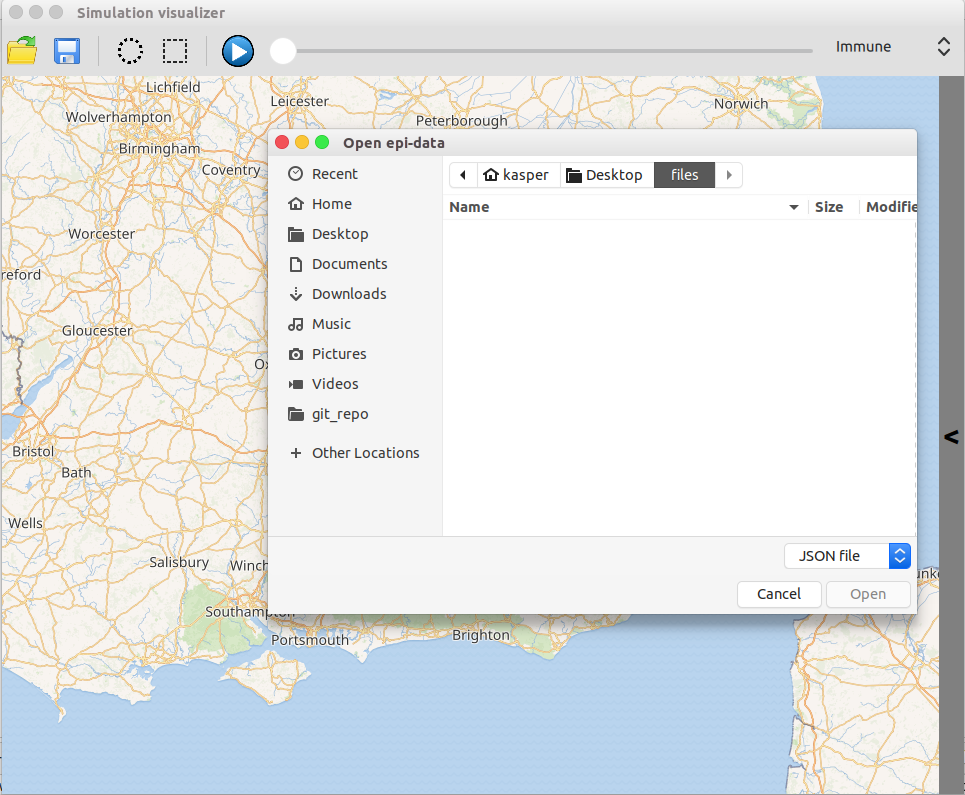
\includegraphics[width=0.7\textwidth,keepaspectratio]{images/open_file.png}
\label{fig:screenshot_openFile}
\caption{The open file dialog}
\end{figure}

Once the file has been opnened, colored circles will appear on the map. The position of each circle corresponds with the geographical location on the map, the color of the circle corresponds with the fraction of the people at the location that have the selected health status. The health status can be selected with the dropdown in the toolbar. An example of an opened simulation result is shown in figure \ref{fig:screenshot_viewSimul}.

%%% IMAGE: view simulation
\begin{figure}[H]
\centering
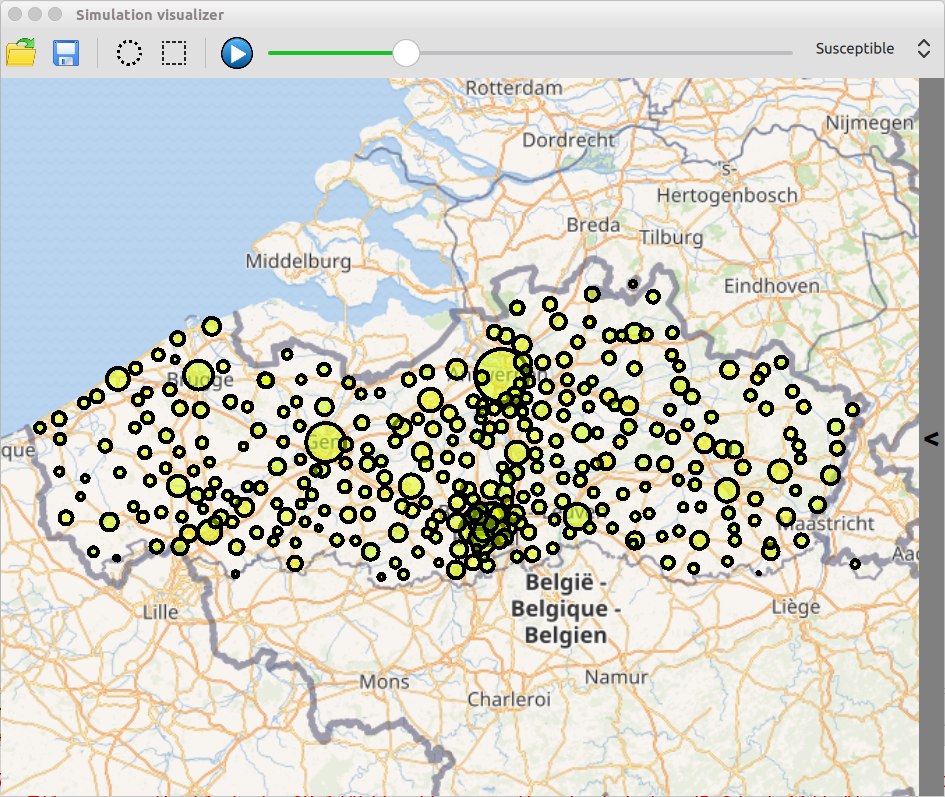
\includegraphics[width=0.7\textwidth,keepaspectratio]{images/view_simul.png}
\label{fig:screenshot_viewSimul}
\caption{The visualiser after a simulation has been opened}
\end{figure}

In order to view a specific timestep of the simulation, the slider in the toolbar can be used. To display an automatic playback of the simulation, the play-pause button can be clicked.

%%%%%%%%%%%%%%%%%%%%%%%%%%%%%%%%%%%%%%%%%%%%%%%%%%%%%%%%%%%%%%%%
% Selecting and viewing statistics
%%%%%%%%%%%%%%%%%%%%%%%%%%%%%%%%%%%%%%%%%%%%%%%%%%%%%%%%%%%%%%%
\section{Selecting and viewing statistics}
\label{section:stats_selection}

Each location on the map contains a set of statistics that indicate how much each subpopulation of the location is affect by the different health statuses. To view these statistics the user has to click on a location and fold open the sidebar. The sidebar will then contain a list of statistics. Such a sidebar can be seen in figure \ref{fig:sceenshot_statsLoc}.

%%% IMAGE: view location stats
\begin{figure}[H]
\centering
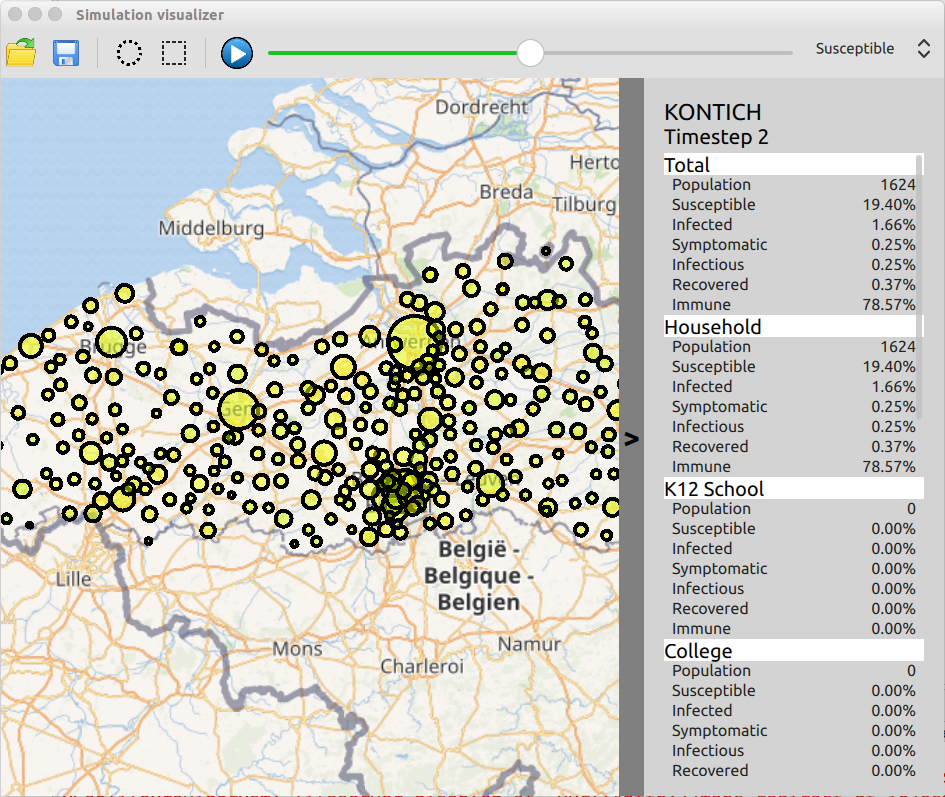
\includegraphics[width=0.7\textwidth,keepaspectratio]{images/stats_loc.png}
\label{fig:sceenshot_statsLoc}
\caption{The sidebar displaying statistics for the clicked location}
\end{figure}

The user may also want to view the statistics of not just one location, but multiple locations combined. To achieve this, the user can click one of the two selection buttons in the toolbar. When the such a button is clicked, a selection dialog will then popup and areas of the map can be selected with the right mouse button. Once the user has made a selection, the confirmation button can be clicked. The results of the selection will then appear in the sidebar. There are two ways to make a selection: rectangular selection (figure \ref{fig:screenshot_selectRect}) and circular selection (figure \ref{fig:screenshot_selectRad}).

%%% IMAGE rect selection
\begin{figure}[H]
\centering
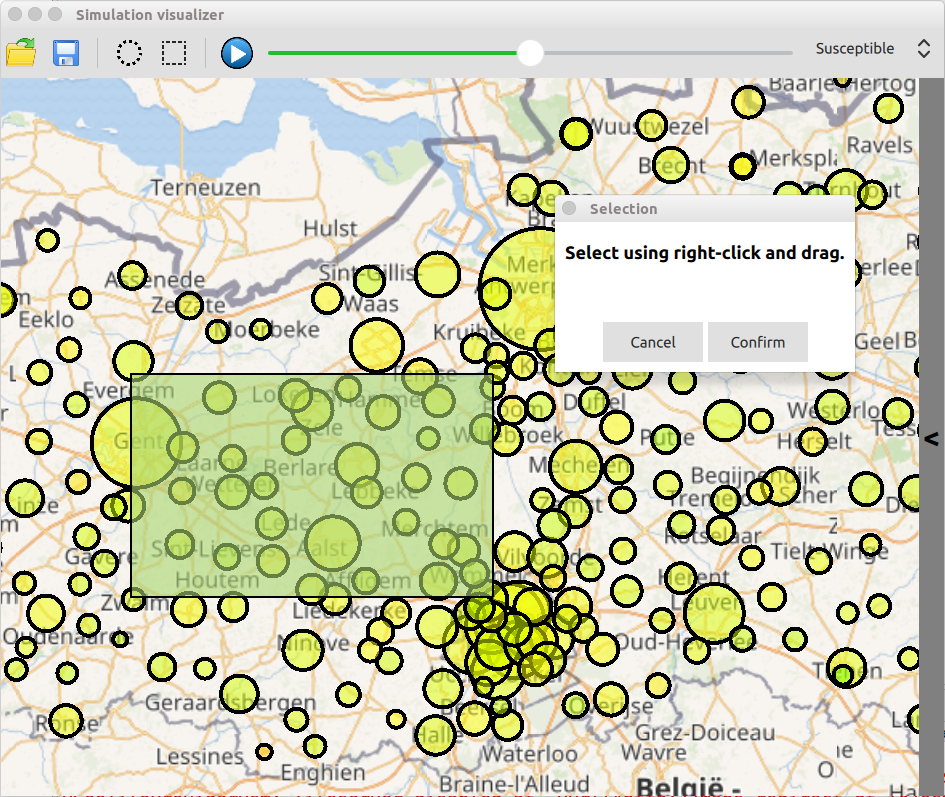
\includegraphics[width=0.7\textwidth,keepaspectratio]{images/select_rect.png}
\label{fig:screenshot_selectRect}
\caption{Rectangular selection}
\end{figure}

%%% IMAGE rad selection
\begin{figure}[H]
\centering
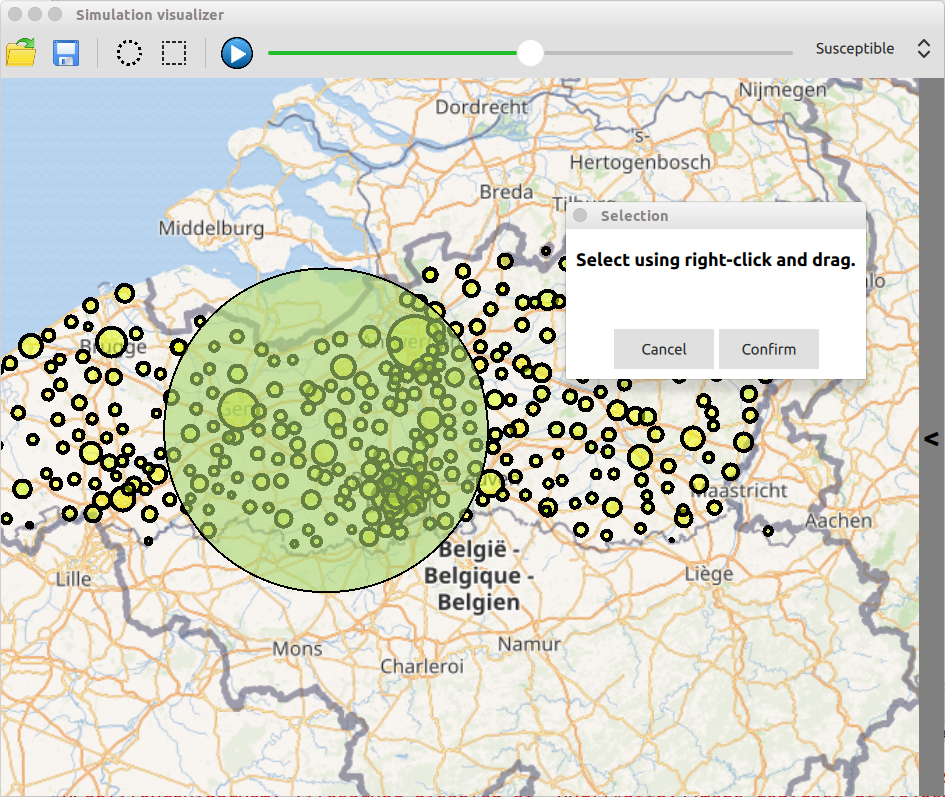
\includegraphics[width=0.7\textwidth,keepaspectratio]{images/select_rad.png}
\label{fig:screenshot_selectRad}
\caption{Radius selection}
\end{figure}


%%%%%%%%%%%%%%%%%%%%%%%%%%%%%%%%%%%%%%%%%%%%%%%%%%%%%%%%%%%%%%%%
% Exporting to image
%%%%%%%%%%%%%%%%%%%%%%%%%%%%%%%%%%%%%%%%%%%%%%%%%%%%%%%%%%%%%%%%

%%% IMAGE save to selection

\section{Exporting to image}
\label{section:export_image}

The visualiser provides the functionality to save the current contents of the map to a PNG file. To do this, the save file button must be clicked, and a save file dialog will open. The user can then select the location in the filesystem where the image will be saved. Such a dialog can be seen in figure \ref{fig:screenshot_saveFile}.

%%% IMAGE save file
\begin{figure}[H]
\centering
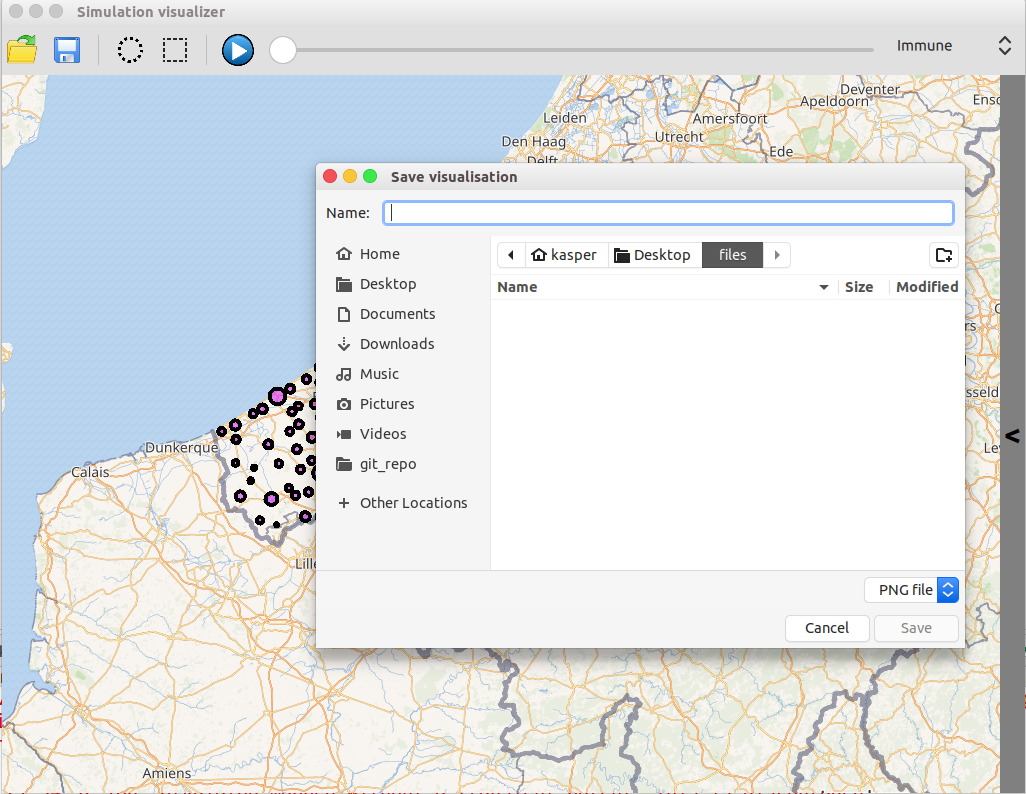
\includegraphics[width=0.7\textwidth,keepaspectratio]{images/save_file.png}
\label{fig:screenshot_saveFile}
\caption{Save to image file}
\end{figure}

